\Chapter{Koncepció}

\Section{Kétkerekű modell kanyarodási íve}

Érdemes lehet előrször a kétkerekű modellt megvizsgálnunk, ugyanis az itt meghatározott képletek adják alapul a négykerekű változatnál használt formulákat.
A kétkerekű (bicikli) modell kanyarodási ívének meghatározása 2 dologtól függ:\newline
\phantom{asd} - a tengelytávolságtól (w),\newline
\phantom{asd} - az első kerék kanyarodási szögétől ($\alpha$).\newline
Az első és hátsó kerekek is egy-egy körpályát fognak követni azonos középponttal. Az irány mindig merőleges a sugárra.

\begin{figure}[h!]
\centering
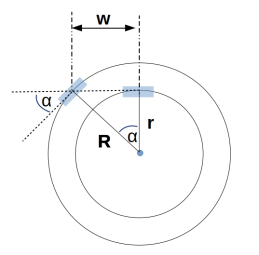
\includegraphics[scale=0.5]{images/two_wheels_rad.png}
\caption{Kétkerekű jármű kanyarodási íve}
\label{fig:two_wheels_rad}
\end{figure}
Az ábrán R az első kerékhez tartozó sugár, r pedig a hátsó kerékhez.\newline
Az első kerék pályája: $\sin\alpha$ = $\cfrac{w}{R}$ \hspace{5mm}---> \hspace{5mm} $R$ = $\cfrac{w}{\sin\alpha}$ \newline
A hátsó kerék pályája: $\tan\alpha$ = $\cfrac{w}{r}$ \hspace{5mm}---> \hspace{5mm} $r$ = $\cfrac{w}{\tan\alpha}$
\newpage


\Section{A jármű matematikai modellje}

Áttérve a négykerekű járművekre szintén meg lehet határozni mind a négy kerékhez tartozó sugarat. A képletek a következők:
$\newline$
$R_{IF}$ =  $\cfrac{w}{\sin\alpha_1}$ - $\cfrac{a}{2}$\newline
$R_{IR}$ =  $\cfrac{w}{\tan\alpha_1}$ - $\cfrac{a}{2}$\newline
$R_{OF}$ =  $\cfrac{w}{\sin\alpha_2}$ + $\cfrac{a}{2}$\newline
$R_{OR}$ =  $\cfrac{w}{\sin\alpha_1}$ + $\cfrac{a}{2}$\newline

Itt az első kerekeknél a sugár az átfogót képezné, míg a hátsó kerekeknél a szög melletti befogót. Ezért is váltakozik a a $\sin$ és a $\tan$ a trigonometriai összefüggések hatására. Az $\cfrac{a}{2}$ pedig attól függően, hogy a kanyarodás irányához viszonyítva a külső vagy belső kerekekről van szó, a tengely hosszának a felét elvesszük vagy hozzáadjuk a képlethez. 

Szeretném egy kicsit részletesebben bemutatni a jármű modelljét és magát a kanyarodási elvet/technológiát. 

A kanyarodás az első kerekek elforgatásával történik. Az első ilyen koncepciónál magát a tengelyt lehetett kormányozni, nem pedig a kerekeket. Ez a megoldás a lassú haladáshoz és a könnyebb manőverezéshez előnyös lehet, de az első tengelynek nagy ívben el kell fordulnia a kanyarodástól függően valamelyik irányba. Ez a futómű kialakítását nagy mértékben korlátozza, maga a felfüggesztés megoldása is nagy kihívás lehet ezt a technológiát használva.

A kanyarodás következő megoldásánál már mindkét első kerék külön-külön forgatható, de azonos az elfordulási szög. Ebben az esetben a jármű dinamikáját nézve úgynevezett oldal irányú csúszás tapasztalható a kerekeken (a kanyarodás irányának függvényében). Ebben közrejátszik, hogy mivel mindkét kerék egy irányba néz ha el van fordítva a kormány, 2 különböző középpontja lesz a forgásnak, így legalább az egyik kerék csúszni fog a kanyarodáskor.

Ideális megoldásnak vesszük azt az esetet, mikor mindkét első kereket egymástól függetlenül lehet kormányozni. Ebben az esetben mindkét kerék kanyarodási szögét meg lehetne úgy határozni, hogy a kerék középpontja egy érintő egyenes lenne a közös kanyarodási középpontból húzható körívre. Így megválasztva a megfelelő sugárt a körívnek, mindkét kereket tekintve elkerülhető az oldal irányú csúszás. A fejezet további ehhez kapcsolódó pontjai is ezt a megoldást fogják tovább részletezni.


Definiálnunk kell különböző jelöléseket, melyek segítségével a képletek leírhatók és értelmezhetők. A négykerekű jármű középpontjának a hátsó tengely középpontját tekintjük. Legalábbis a z elforduláshoz szükséges számításoknál ezt vesszük figyelembe. Mivel a kanyarodásnál az első kerekek különböző szögeket zárnak be az első tengellyel, ezért érdemes egy képzeletbeli, az első tengely közepére eső kormányozható kereket megadni. Ennek a jármű irányával bezárt előjeles szögét jelöljük $\alpha$-val. A jármű tengelytávolságát jelöljük $w$-vel, a hátsó tengely hosszát pedig $a$-val (\ref{fig:vehicle}. ábra).

\begin{figure}[h!]
\centering
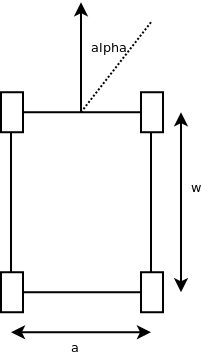
\includegraphics[scale=0.45]{images/vehicle.png}
\caption{A jármű matematikai modelljének fő paraméterei}
\label{fig:vehicle}
\end{figure}

\Section{Első kerekek elfordulási szögének kiszámítása}

A kanyarodásnál tehát figyelembe kell venni, hogy a két első kerék különböző szögben fordul el, mégpedig az iránytól függően a belső kerék nagyobb szögben tér el az egyenestől, míg a külső kisebb szögben. Minél nagyobb a kanyarodási szög, annál nagyobb az eltérés a két kerék elfordulásában.
Az $\alpha$ szög függvényében külön ki kell számítanunk a jármű bal és jobb első kerekének elfordulási szögét.
Tehát első lépésben határozzuk meg az adott $\alpha$ szög ismeretében a további számításokhoz szükséges sugarat,
melyet a \ref{fig:turning_vehicle}. ábrán R jelöl. Ez a kanyarodási sugár, melyet a jármű középvonalához mérünk.
Az ehhez szükséges képlet:\vspace{2mm}
$R$ = $\dfrac{w}{\text{tg} \alpha}$ \vspace{5mm}

Továbbiakban a jelölések ugyanazok, az első kerekeket tekintve pedig $\alpha_1$ a belső, $\alpha_2$ pedig a külső kerék elfordulási szögét jelöli.  
A jármű tengelytávolsága, valamint szélessége, és a sugár ismeretében ezen két szög a következőképpen számítható ki:\vspace{5mm}

$\alpha\textsubscript{1}$ = $\text{arctan}\Bigg(\cfrac{w}{R-\frac{a}{2}}\Bigg)$ \hspace{1cm} $\alpha\textsubscript{2}$ = $\text{arctan}\Bigg(\cfrac{w}{R+\frac{a}{2}}\Bigg)$\vspace{5mm}

A kanyarodási sugárból átalakítható a képlet a trigonometrikus összefüggéseket figyelembe véve. A szögeket megkaphatjuk, ha a képletet rendezzük úgy, hogy a tangens inverzével szorozva elosztjuk a tengelytávolságot az adott kerékhez tartozó sugárral. Ugyanis az arctan visszaadja azt a szöget, ami jelen esetben a sugárhoz és a tengelytávolsághoz tartozik. Mivel mindkét keréknek más lesz a sugara a kijelölt ponttól, ezeket is is külön meg kell határozni, így a képlet nevezőjében a kanyarodási középponthoz közelebb eső kerékhez tartozó sugárból kivonjuk a jármű szélességének felét, míg a messzebb eső kerékhez hozzáadjuk ezt az értéket.

\begin{figure}[h!]
\centering
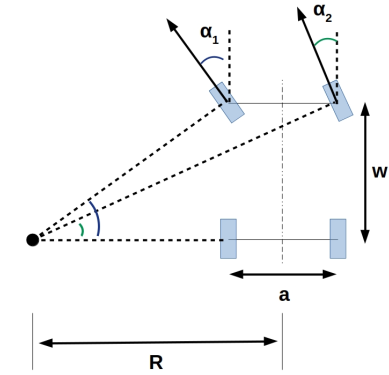
\includegraphics[scale=0.5]{images/turning_vehicle.png}
\caption{Első kerekek elfordulási szögei}
\label{fig:turning_vehicle}
\end{figure}


% TODO: Részletesen leírni ezek számítását!

\Section{Pozíció számítása rögzített $\alpha$ mellett}

A rögzített $\alpha$ szög, és adott sebesség mellett ki kell tudnunk számolni, hogy adott $(x_0, y_0)$ kiindulópontból indulva a jármű milyen pozícióba fog kerülni $t$ idő elteltével. Az $\alpha$ szög függvényében az alábbi módon számolhatjuk ki annak a képzeletbeli körnek a sugarát ($R$), amelyen a jármű majd kanyarodni fog:
\[
R = \dfrac{w}{\text{tg} \alpha},
\]
ahol a $w$ a jármű tengelyei közötti távolságot jelöli.

Tegyük fel, hogy a jármű sebessége $v$. Ekkor $t$ idő függvényében a jármű pozícióját az alábbi formában számolhatjuk:
\begin{align*}
x(t) &= x_0 + R - R \cdot \cos \dfrac{v \cdot t}{|R|}, \\
y(t) &= y_0 + |R| \cdot \sin \dfrac{v \cdot t}{|R|}.
\end{align*}

\Section{Útvonal meghatározása az eltelt idő függvényében}

$$
\vec{v} \in \mathbb{R} \hspace{0.5cm}
\quad \rightarrow \quad
\vec{v} (t) \colon \mathbb{R} \to \mathbb{R}^2
$$

Elfordulás:
$$
\varphi (t) \hspace{0.5cm} \rightarrow \hspace{0.5cm} \vec{v} (t) =
\begin{bmatrix}
\cos(\varphi(t)) \\
\sin(\varphi(t))
\end{bmatrix}
$$

$ \vec{x_0} $ : kezdőpozíció

Egy egységnyi idő elteltével az irány: $ \vec{x} (t_1) = \vec{x_0} + \displaystyle\int_{t_0}^{t_1} \vec{v} (t) dt $

Általános alak:  $ \vec{x} (t) = \vec{x_0} + \displaystyle\int_{t_0}^{t} \vec{v} (u) du $

$$
\begin{bmatrix} x_1 \\ y_1 \end{bmatrix} = \begin{bmatrix} x_0 \\ y_0 \end{bmatrix} + \displaystyle\int_{t_0}^{t_1} \begin{bmatrix} \cos(\varphi(t)) \\ \sin(\varphi(t)) \end{bmatrix} dt 
$$


Külön a két vektort leintegráljuk:
\begin{align*}
x_1 &= x_0 + \displaystyle\int_{t_0}^{t_1} \cos(\varphi(t)) \; \mathrm{d}t \\ \\
y_1 &= y_0 + \displaystyle\int_{t_0}^{t_1} \sin(\varphi(t)) \; \mathrm{d}t \\
\end{align*}

Az integrálás kifejtése:
\begin{align*}
x_1 = x_0 + \left[\dfrac{1}{\varphi} \cdot \sin(\varphi(t))\right]_{t_0}^{t_1} = x_0 + \left(\left(\dfrac{1}{\varphi} \cdot \sin(\varphi({t_1)})\right) - \left(\dfrac{1}{\varphi} \cdot \sin(\varphi({t_0}))\right)\right)  \\ \\
y_1 = y_0 + \left[- \dfrac{1}{\varphi} \cdot \cos(\varphi(t))\right]_{t_0}^{t_1} = y_0 + \left(\left(- \dfrac{1}{\varphi} \cdot \cos(\varphi({t_1)})\right) - \left(- \dfrac{1}{\varphi} \cdot \sin(\varphi({t_0}))\right)\right) \\
\end{align*}

Ezzel a számítással megkaphatjuk a jármű által bejárt utat. Jelen esetben a képlet mindig csak a következő pozítiót adja meg, tehát $x_1$ jelentené a következő pozíciót, $x_0$ az előzőt. Az idő szintén a nulladik és az első időpillanatra vonatkozik ($t_0$, $t_1$), valamint a kanyarodási szög mindig az aktuális. Ennek a szögnek az értékénél figyelembe kell venni, hogy negatív vagy pozitív szám. Ez megadja, hogy melyik irányba kanyarodik a jármű a 0 fokhoz képest (ami azt jelenti, hogy előre felé néz). Ha a $\varphi$ < 0 akkor jobbra, ha $\varphi$ > 0  akkor balra fog kanyarodni. 

\end{document}


